\subsection{Implementation Plan}
For the implementation phase of our project we decided to follow a bottom-up strategy. In particular, starting from the Data4Help subsystem, we will implement each component separately and then perform unit tests on it. By adopting this strategy we incrementally develop working components.
As it concerns the implementation order, we decided to start from the Data4Help back-end module, since we think is the most critical one because the other two subsystems work on top of it.
In a second time, developer SDKs should be completed before the other two subsystem's back-end development can be carried out.
Finally, we can integrate front-ends in all our subsystems.
The order could be the following:

\begin{enumerate}
    \item Data4Help back-end
    \item Third Party SDK
    \item Data Source SDK
    \item Automated SOS and Track4Run back-ends
    \item Data4Help front-end
    \item AutomatedSOS and Track4Run front-ends
\end{enumerate}

\subsubsection{Data4Help Basic Back-End}
The first components to be developed should be the ones that guarantee the basic Data4Help back-end functions, which means all the services that are related to data acquisition and data requests. Here is a diagram representing a possible order in which these components should be developed. As already stated, after each development phase a \textit{Unit Test} phase and an \textit{Integration Test} phase should follow, in order to validate the new component and verify its integration with the previously developed system.

\FloatBarrier
\begin{figure}[!h]
	\centering
	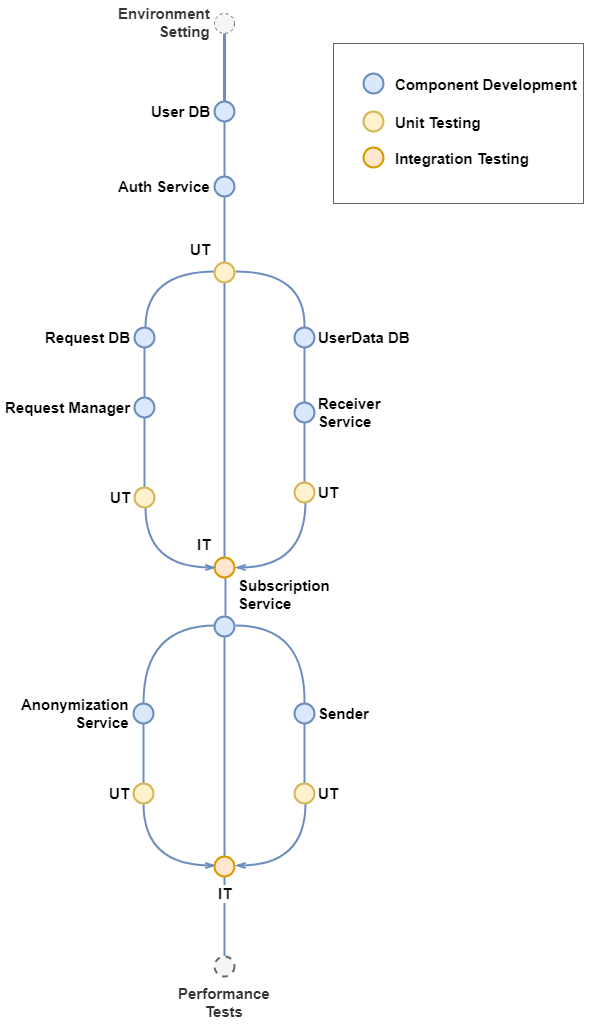
\includegraphics[width=0.7\columnwidth]{d4h_dev.png}
	\caption{Data4Help Development Plan}
\end{figure}
\FloatBarrier

\subsubsection{Developer's SDKs}
The Third Party SDK and Data Sources SDK must be carried out after Data4Help basic back-end is completed and before developing other back-ends. This will guarantee that AutomatedSOS and Track4Run subsystems will be able to properly interact with the Data4Help APIs.

In particular, there is no dependency between the two SDKs, but certainly the Third Party SDK is the most important one in this phase, since AutomatedSOS and Data4Help development depend upon it. Anyway the development of these two subsystems can start independently, and we can integrate these SDKs in a second moment.

\subsubsection{AutomatedSOS and Track4Run Back-Ends}
After the SDKs are developed, the remaining two subsystems' back-ends can be developed in a fully parallel line. Like in the case of Data4Help, an incremental approach is recommended in these development phases, and Unit and Integration tests should be performed at every step.

\FloatBarrier
\begin{figure}[!h]
	\centering
	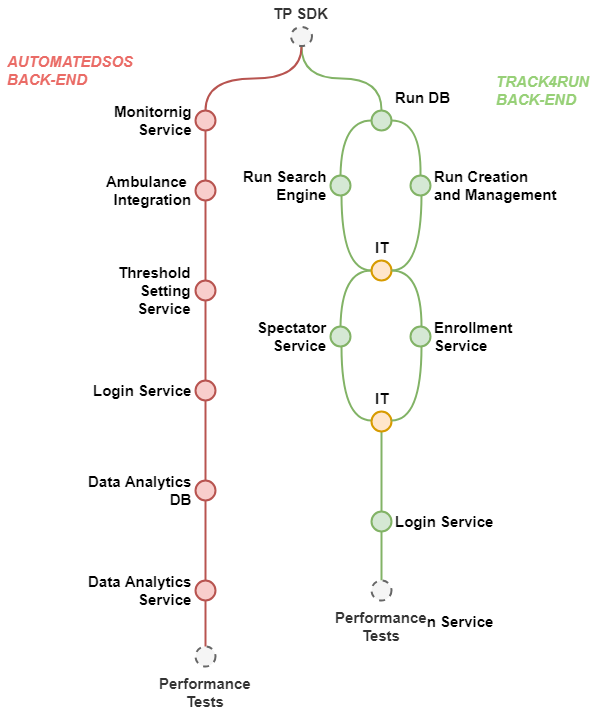
\includegraphics[width=0.9\columnwidth]{other_be_dev.png}
	\caption{Data4Help Development Plan}
\end{figure}
\FloatBarrier

\subsubsection{Front-Ends and External Services Integration}
Finally we can develop the front-ends and integrate the subsystems with the external services. Each front-end is obviously independent from the others, and the external service integration can as well be performed separately for each subsystem.

\begin{itemize}
	\item \textbf{Data4Help}
\end{itemize}

\FloatBarrier	
\begin{figure*}[ht!]	
	\centering	
	\begin{subfigure}[t]{0.5\textwidth}	
		\centering	
		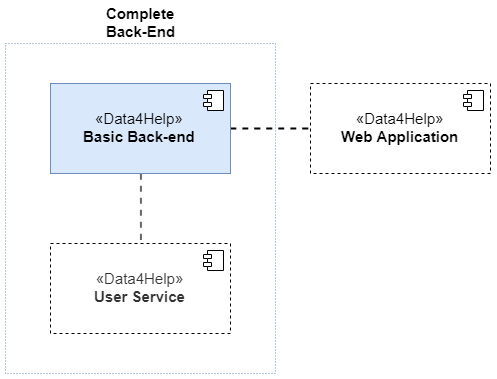
\includegraphics[width=\columnwidth]{d4h_int1.png}	
		\caption{Stage I}	
	\end{subfigure}%	
	~ \vspace{20px}	
	\begin{subfigure}[t]{0.5\textwidth}	
		\centering	
		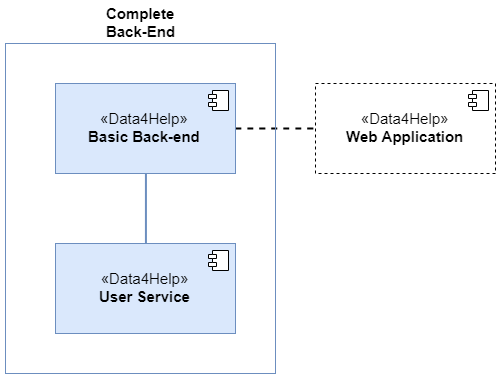
\includegraphics[width=\columnwidth]{d4h_int2.png}	
		\caption{Stage II}	
	\end{subfigure}	
	\begin{subfigure}[t]{0.5\textwidth}	
		\centering	
		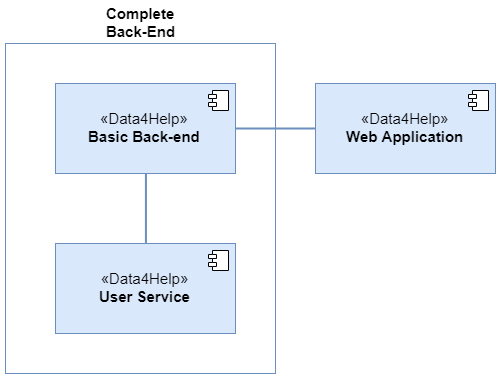
\includegraphics[width=\columnwidth]{d4h_int3.png}	
		\caption{Stage III}	
	\end{subfigure}	
	
	\caption{Data4Help Front-End Integration Steps}	
\end{figure*}	

\FloatBarrier
	
\begin{itemize}
	\item \textbf{AutomatedSOS}
\end{itemize}

\FloatBarrier
\begin{figure*}[ht!]	
	\centering	
	\begin{subfigure}[t]{0.5\textwidth}	
		\centering	
		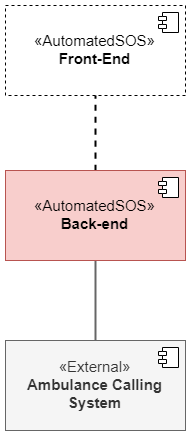
\includegraphics[width=0.5\columnwidth]{autosos_int1.png}	
		\caption{Stage I}	
	\end{subfigure}%	
	~ \vspace{20px}	
	\begin{subfigure}[t]{0.5\textwidth}	
		\centering	
		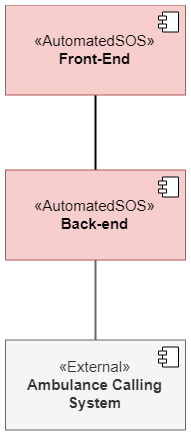
\includegraphics[width=0.5\columnwidth]{autosos_int2.png}	
		\caption{Stage II}	
	\end{subfigure}	
	\caption{AutomatedSOS Final Integration Steps}	
\end{figure*}	
\FloatBarrier

\begin{itemize}
	\item \textbf{Track4Run}
\end{itemize}


\FloatBarrier
\begin{figure*}[ht!]	
	\centering	
	\begin{subfigure}[t]{0.3\textwidth}	
		\centering	
		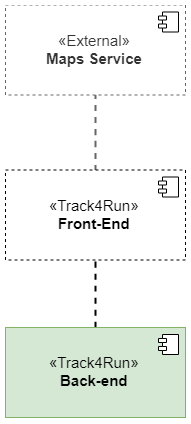
\includegraphics[width=0.8\columnwidth]{t4r_int1.png}	
		\caption{Stage I}	
	\end{subfigure}%		
	~ \vspace{20px}	
	\begin{subfigure}[t]{0.3\textwidth}	
		\centering	
		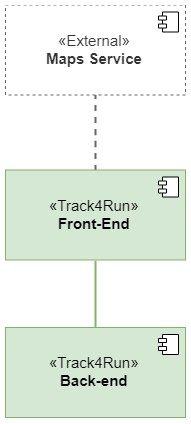
\includegraphics[width=0.8\columnwidth]{t4r_int2.png}	
		\caption{Stage II}	
	\end{subfigure}
	~ \vspace{20px}
	\begin{subfigure}[t]{0.3\textwidth}	
		\centering	
		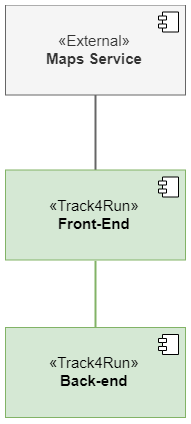
\includegraphics[width=0.8\columnwidth]{t4r_int3.png}	
		\caption{Stage III}	
	\end{subfigure}	
	
	\caption{Track4Run Final Integration Steps}	
\end{figure*}	
\FloatBarrier

\subsection{Integration and Testing}
\subsubsection{Integration Testing Strategy}
With respect to the integration between developed components, we decided to follow a \textit{continuous integration} strategy: as soon as a first version of a component is released, we need to test it and then integrate it with the already existing components of the system. This strategy has been chosen because it enables the developers to have many checkpoints where they can test their product and makes it easy to find bugs early in the development of the system, so that if things break, they break small.

Once each back-end have been completely developed and integrated, it's also highly recommended to carry out a system testing process. In particular:

\begin{itemize}
    \item \textbf{Performance Testing:} for each subsystem, we need to monitor the responsiveness of the services with respect to incoming requests. In particular, Data4Help should be very fast in managing new data samples to guarantee a fluid service to the third-parties. In addition, AutomatedSOS needs to be extremely fast in detecting and responding to an emergency due to the 5 seconds time constraint. Lastly, Track4Run user experience is heavily influenced by the back-end performances, which should be for this reason flawless.
    \item \textbf{Load Testing:} after the performance testing, is suggested to continuously feed each subsystem with an increasing number of requests. This is done to assess the performances and availability of each subsystem in case of unusually high volumes of incoming requests. This phase also tells us if the system can handle malicious attacks which try to exploit memory leaks, buffer overflows and similar bugs.  
    \item \textbf{Stress Testing:} finally, in order to test if the subsystems are able to recover from unexpected failures, we should simulate them in a controlled manner.
\end{itemize}

\subsubsection{Entry Criteria}
As stated above, continuous integration forces the testing phase to start as soon as a component is merged with the main product. However, it is necessary to be sure that a correct environment is setup before integration can be effectively carried out. In particular, in case of Data4Help we need the following components:

\begin{itemize}
    \item \textit{Microservices Containers}
    \item \textit{API Gateway}
    \item \textit{Message Queue Server}
    \item \textit{Service Registry}
    \item \textit{DataBase Managment System}
    \item \textit{Performance Monitor}
\end{itemize}

For AutomatedSOS and Track4Run instead we need the web server and firewalls to be correctly set-up and the \textit{Third-Party SDK} to be available and already tested against the Data4Help request APIs.

\subsubsection{Elements to be Integrated}
As seen in the development plan, we can divide our components in groups considering the existing dependencies between them. The following diagrams are meant to clarify these dependencies:

\FloatBarrier
\begin{figure}[!h]
	\centering
	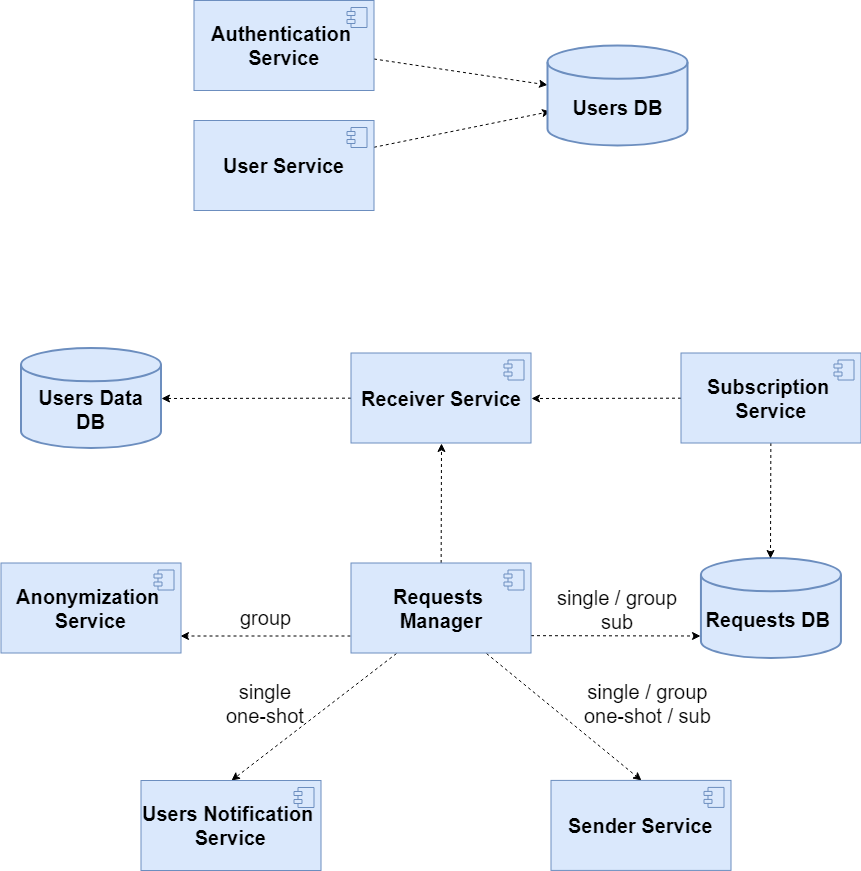
\includegraphics[width=0.7\columnwidth]{dependenciesDiagram-Data4Help.png}
	\caption{Data4Help Components Dependencies}
\end{figure}
\FloatBarrier

\FloatBarrier
\begin{figure}[!h]
	\centering
	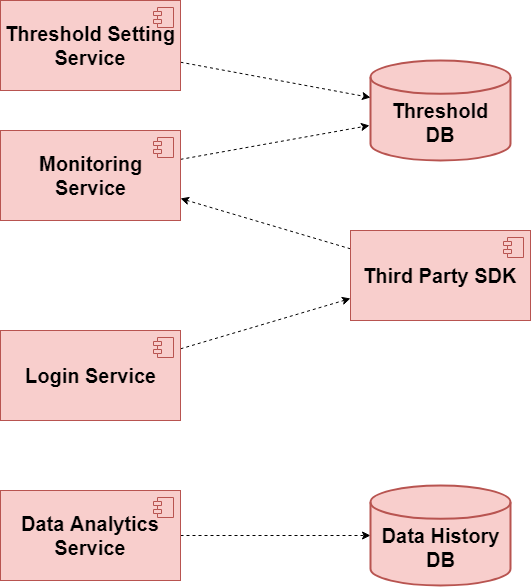
\includegraphics[width=0.7\columnwidth]{dependenciesDiagram-AutomatedSOS.png}
	\caption{AutomatedSOS Components Dependencies}
\end{figure}
\FloatBarrier

\FloatBarrier
\begin{figure}[!h]
	\centering
	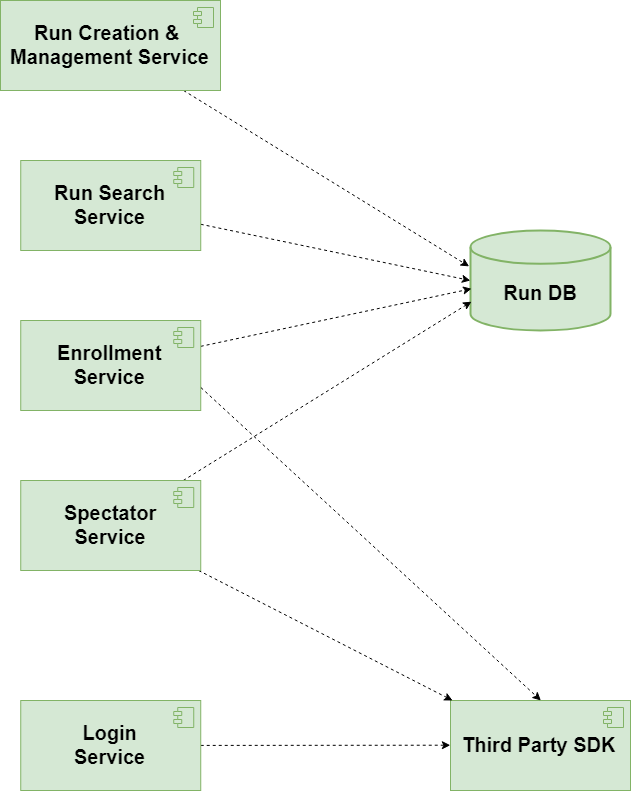
\includegraphics[width=0.7\columnwidth]{dependenciesDiagram-Track4Run.png}
	\caption{Track4Run Components Dependencies}
\end{figure}
\FloatBarrier

\subsubsection{Sequence of Component/Function Integration}
Since we adopted a continuous integration strategy, the integration phase runs in parallel  with the implementation phase, which is carefully described in the previous diagrams.
